\documentclass[11pt]{article}

\usepackage[margin=1in]{geometry}
\usepackage{amsmath,amssymb}
\usepackage{mathtools}
\usepackage{booktabs}
\usepackage{graphicx}
\usepackage{float}
\usepackage{hyperref}

\newcommand{\dg}{^{\dagger}}
\newcommand{\ket}[1]{|#1\rangle}
\newcommand{\bra}[1]{\langle #1|}
\newcommand{\braket}[1]{\langle #1\rangle}
\newcommand{\Tr}{\mathrm{Tr}}

\title{The $t_c$-Cederbaum model: ghost Gutzwiller by direct minimization\\
\large (core fragment with $B_c=1$, $3$ and $5$ quasiparticle orbitals)}
\author{}
\date{\today}

\begin{document}
\emergencystretch=4em
\maketitle

\noindent This note defines the Hamiltonian that is solved, the $t_c$-Cederbaum model (the Cederbaum model of core-hole satellites plus a weak
core--virtual hopping $t_c$; $t_c=0$ is the original Cederbaum model), its exact solution by diagonalization (ED), the
ghost-Gutzwiller (gGut) variational problem used for it, the direct minimization that solves that problem, and the
comparison of the gGut results with ED, for a core fragment without ghosts ($B_c=1$) and with two and four ghosts
($B_c=3$, $5$). The aim of the test is to see whether gGut reproduces the satellite structure of the core-hole spectrum of this model.
Quantities are per spin unless stated otherwise; solutions are real and paramagnetic.

%======================================================================
\section{The Hamiltonian}
\label{sec:H}

Three orbitals, $c$ (core), $o$ (occupied) and $v$ (virtual), each with two spins. The $t_c$-Cederbaum model is
$H_{\rm tot}=H+H_t$, where $H$ is the Cederbaum model (the $o$--$v$ hopping conditioned on a core hole) and $H_t$ the added hopping:
\begin{equation}
\begin{aligned}
H_{\rm tot}={}&g\sum_\sigma(n_{v\sigma}-n_{o\sigma})-E_c\sum_\sigma n_{c\sigma}
-V\sum_{\sigma\sigma'}(1-n_{c\sigma})\left(c\dg_{v\sigma'}c_{o\sigma'}+\mathrm{h.c.}\right)\\
&+t_c\sum_\sigma\left(c\dg_{c\sigma}c_{v\sigma}+\mathrm{h.c.}\right),
\end{aligned}
\label{eq:Htot}
\end{equation}
with $E_c>0$, orbital gap $g$, core--valence coupling $V$, and a weak core--virtual hopping $t_c$. The prefactor
$\sum_\sigma(1-n_{c\sigma})=2-n_c$ counts the core holes, so the $o$--$v$ hopping acts only when the core is not full.
The particle number and $S_z$ are conserved. The core occupation $n_c$ is conserved only at $t_c=0$. Energies are measured in units of $g$ ($g=1$), so the parameters are the ratios $E_c/g$, $V/g$ and $t_c/g$. All results
below use $E_c/g=10$, $V/g\in\{1/\sqrt2,\sqrt2\}=\{0.707,1.414\}$ and $t_c/g\le0.5$; the ground state then lies in the sector with two electrons of each
spin. The two values of $V$ are chosen so that $\rho/\Omega=V/(\sqrt2\,g)=0.5$ and $1.0$, the ratios of the transition moment $\rho$ to the excitation
energy $\Omega=2g$ used by Kockl\"auner and Golze for this model~\cite{Kocklauner2024} (Sec.~\ref{sec:golze}); $E_c$ only shifts all poles rigidly at $t_c=0$.

%======================================================================
\section{Exact diagonalization}
\label{sec:ED}

\paragraph{Diagonalization.} $H_{\rm tot}$ is diagonalized exactly in the 64-dimensional Fock space of six spin orbitals
(Jordan--Wigner operators). At $t_c=0$ the ground state is the product state $\ket{220}$
(notation $\ket{n_cn_on_v}$: core and $o$ doubly occupied, $v$ empty) with $E=-2E_c-2g$ and core occupation $\nu_c=\braket{n_c}=2$; for $t_c>0$ it acquires a
core-hole component and $\nu_c<2$. The core-hole Green's function for spin $\uparrow$ is
\begin{equation}
G^h_{cc}(\omega)=\sum_n\frac{|\braket{n|c_{c\uparrow}|{\rm GS}}|^2}{\omega+(E_n-E_{\rm GS})-i\eta},
\label{eq:Gh}
\end{equation}
with poles at $\omega=-E_i$ and weights $p_i$. At $t_c=0$ there are three poles; with $\alpha=V/g$,
\begin{equation}
\begin{aligned}
E_1&=E_c+2g-2g\sqrt{1+\alpha^2}, & p_1&=\frac{(1+\sqrt{1+\alpha^2})^2}{4(1+\alpha^2)},\\
E_2&=E_c+2g, & p_2&=\frac{\alpha^2}{2(1+\alpha^2)},\\
E_3&=E_c+2g+2g\sqrt{1+\alpha^2}, & p_3&=\frac{(1-\sqrt{1+\alpha^2})^2}{4(1+\alpha^2)},
\end{aligned}
\label{eq:poles}
\end{equation}
which the ED reproduces to $9\times10^{-15}$. For $t_c>0$ the poles move at $O(t_c^2)$ and the middle pole splits into two
lines $\sim10^{-4}$ apart (Tab.~\ref{tab:EDpoles}); Tab.~\ref{tab:ED} gives the ground-state quantities.

\begin{table}[h]
\centering
\small
\begin{tabular}{rrrrr}
\toprule
$V/g$ & $t_c/g$ & $(E_0+2E_c+2g)/g$ & $2-\nu_c$ & $\rho^{cv}=\braket{c\dg_{c\uparrow}c_{v\uparrow}}$\\
\midrule
0.707 & 0.5  & $-4.55\times10^{-2}$ & $4.15\times10^{-3}$ & $-4.54\times10^{-2}$\\
0.707 & 0.2  & $-7.30\times10^{-3}$ & $6.67\times10^{-4}$ & $-1.82\times10^{-2}$\\
0.707 & 0.1  & $-1.82\times10^{-3}$ & $1.67\times10^{-4}$ & $-9.12\times10^{-3}$\\
0.707 & 0.05 & $-4.56\times10^{-4}$ & $4.17\times10^{-5}$ & $-4.56\times10^{-3}$\\
1.414 & 0.5  & $-4.60\times10^{-2}$ & $4.27\times10^{-3}$ & $-4.59\times10^{-2}$\\
1.414 & 0.2  & $-7.37\times10^{-3}$ & $6.87\times10^{-4}$ & $-1.84\times10^{-2}$\\
1.414 & 0.1  & $-1.84\times10^{-3}$ & $1.72\times10^{-4}$ & $-9.22\times10^{-3}$\\
1.414 & 0.05 & $-4.61\times10^{-4}$ & $4.30\times10^{-5}$ & $-4.61\times10^{-3}$\\
\bottomrule
\end{tabular}
\caption{Exact ground state of $H_{\rm tot}$: $2-\nu_c\propto t_c^2$ and $\rho^{cv}\propto t_c$.}
\label{tab:ED}
\end{table}

\begin{table}[h]
\centering
\small
\begin{tabular}{r l rrr r}
\toprule
$V/g$ & & $-E_1$ & $-E_2$ (split pair) & $-E_3$ & $p_1$\\
\midrule
0.707 & $t_c\to0$ (Eq.~\ref{eq:poles}) & $-9.5505$ & $-12$ & $-14.4495$ & $0.8249$\\
      & $t_c/g=0.5$  & $-9.5777$ & $-12.0441,\,-12.0477$ & $-14.5121$ & $0.8268$\\
      & $t_c/g=0.1$  & $-9.5516$ & $-12.0018,\,-12.0019$ & $-14.4520$ & $0.8250$\\
      & $t_c/g=0.05$ & $-9.5508$ & $-12.0004,\,-12.0005$ & $-14.4501$ & $0.8249$\\
\midrule
1.414 & $t_c\to0$ (Eq.~\ref{eq:poles}) & $-8.5359$ & $-12$ & $-15.4641$ & $0.6220$\\
      & $t_c/g=0.5$  & $-8.5707$ & $-12.0406,\,-12.0510$ & $-15.5198$ & $0.6263$\\
      & $t_c/g=0.1$  & $-8.5373$ & $-12.0016,\,-12.0020$ & $-15.4663$ & $0.6222$\\
      & $t_c/g=0.05$ & $-8.5362$ & $-12.0004,\,-12.0005$ & $-15.4647$ & $0.6221$\\
\bottomrule
\end{tabular}
\caption{Exact hole poles of $G^h_{cc}$ at $V/g=0.707$ and $1.414$ (weights $>10^{-3}$); the split pair has total weight $p_2=\alpha^2/[2(1+\alpha^2)]=0.1667$ and $0.3333$, respectively.}
\label{tab:EDpoles}
\end{table}

%======================================================================
\section{The ghost-Gutzwiller variational problem}
\label{sec:gGut}

\paragraph{Fragments and quasiparticle space.} Each orbital $I\in\{c,o,v\}$ is a fragment with $B_I$ quasiparticle
orbitals $d_{Ia\sigma}$, $a=1,\dots,B_I$: $B_o=B_v=1$ (no local interaction) and $B_c\in\{1,3,5\}$, i.e.\ $B_c-1$ ghost orbitals on
the core. The Gutzwiller wave function is $\ket{\Psi_G}=\prod_IP_I\ket{\psi_{qp}}$ with $\ket{\psi_{qp}}$ a Slater determinant that fills
$N_{\rm occ}=2+(B_c-1)/2$ of the $B_c+2$ levels per spin. Its one-body density matrix is
$\rho^{IJ}_{ab}=\braket{d\dg_{Ia\sigma}d_{Jb\sigma}}$.

\paragraph{Embedding states.} The projector of each fragment is represented by a real normalized state $\Phi_I$ in the
Fock space of the physical orbital $I$ plus $B_I$ bath orbitals per spin, restricted to the half-filled sector with
$(1+B_I)/2$ electrons of each spin ($B_I$ odd). Writing $c_{I\sigma}$ for the physical and $d_{Ia\sigma}$ for the bath orbitals, the
following quantities are expectation values in $\Phi_I$ (spin averaged):
\begin{equation}
\begin{aligned}
D_{I,a}&=\tfrac12\sum_\sigma\braket{d\dg_{Ia\sigma}c_{I\sigma}}, &
\Delta^{bb}_{I,ab}&=\tfrac12\sum_\sigma\braket{d\dg_{Ia\sigma}d_{Ib\sigma}},\\
\nu_c&=\braket{n_c}, &
K_{\gamma\delta}&=\Big\langle n_c\sum_\sigma d_{c\delta\sigma}d\dg_{c\gamma\sigma}\Big\rangle,
\end{aligned}
\end{equation}
and $E^{loc}_I=\braket{H^{loc}_I}$ with $H^{loc}_c=-E_cn_c$, $H^{loc}_o=-g n_o$, $H^{loc}_v=+g n_v$
($n_I=\sum_\sigma n_{I\sigma}$). From them:
\begin{equation}
{}^I\Delta=\mathbb I-\Delta^{bb}_I,\qquad S_I=\big[{}^I\Delta(\mathbb I-{}^I\Delta)+\varepsilon\,\mathbb I\big]^{1/2},\qquad
R_I=S_I^{-1}D_I,\qquad C=(\mathbb I-{}^c\Delta+\varepsilon\,\mathbb I)^{-1},
\end{equation}
where $\varepsilon$ is a small regularizing shift ($10^{-9}$ unless stated) and $R_I\in\mathbb R^{B_I}$ is the renormalization vector,
$c\dg_{I\sigma}\to\sum_aR_{I,a}d\dg_{Ia\sigma}$. The non-local core--valence correlation enters through the tensor
\begin{equation}
\bar\Theta=\tfrac12S_c^{-1}KS_c^{-1}-\nu_c\,C,\qquad u=\rho^{cv}R_v,\quad w=\rho^{co}R_o,
\end{equation}
which follows from evaluating $\braket{\Psi_G|n_{c\sigma}c\dg_{o\sigma'}c_{v\sigma'}|\Psi_G}$ with the Gutzwiller approximation
(derived in \texttt{main.tex}, Eqs.~ThetaEff--ThetaEqn, and \texttt{SI.tex}, S2).

\paragraph{Energy functional.} The energy is $E=\braket{\Psi_G|H_{\rm tot}|\Psi_G}$, evaluated term by term from Eq.~\eqref{eq:Htot}
with $c\dg_{I\sigma}\to\sum_aR_{I,a}d\dg_{Ia\sigma}$ and Wick's theorem on $\ket{\psi_{qp}}$.
\begin{itemize}
\item \emph{Local terms.} $g(n_v-n_o)-E_cn_c=\sum_IH^{loc}_I$ is evaluated in the embedding states, $\sum_IE^{loc}_I$.
\item \emph{Core--virtual hopping.} Per spin, $\braket{c\dg_{c\sigma}c_{v\sigma}}=R_c^T\rho^{cv}R_v$. The sum over the two spins and the
hermitian conjugate give a factor $4$: $\;4t_c\,R_c^T\rho^{cv}R_v$.
\item \emph{Conditioned $o$--$v$ hopping.} The weight $(2-n_c)$ multiplies $\sum_{\sigma'}(c\dg_{v\sigma'}c_{o\sigma'}+\mathrm{h.c.})$ and the expectation
value does not factorize, since $n_c$ fluctuates and is correlated with the hopping. Per spin,
$\braket{(2-n_c)\,c\dg_{v\sigma}c_{o\sigma}}=(2-\nu_c)\,R_v^T\rho^{vo}R_o+w^T\bar\Theta\,u$: the first part is the mean-field one, with the average
number of core holes $2-\nu_c$; the second is the connected core--valence correlation, built from $\bar\Theta$, $u$ and $w$ defined above.
Spin sum and hermitian conjugate again give a factor $4$.
\end{itemize}
Adding the three contributions with the prefactors of Eq.~\eqref{eq:Htot}:
\begin{equation}
E=\underbrace{\sum_IE^{loc}_I}_{\rm local}+\underbrace{4t_c\,R_c^T\rho^{cv}R_v}_{t_c\ \rm hopping}
-\underbrace{4V(2-\nu_c)\,R_v^T\rho^{vo}R_o}_{o\text{--}v\ \rm mean\ field}-\underbrace{4V\,w^T\bar\Theta\,u}_{\rm connected}.
\label{eq:E}
\end{equation}
Written out with the definitions above, the dependences are: $E^{loc}_I$, $\nu_c$, $\Delta^{bb}_I$ and $K$ are expectation values in
$\Phi_I$; $R_I=S_I^{-1}D_I$ with $S_I$ a function of $\Delta^{bb}_I$; $\bar\Theta$ a function of $\nu_c$, $K$ and ${}^c\Delta$;
$u=\rho^{cv}R_v$ and $w=\rho^{co}R_o$. So $E$ depends on the embedding states only through $E^{loc}_I$, $D_I$, $\Delta^{bb}_I$, $\nu_c$ and
$K$, and on $\ket{\psi_{qp}}$ only through $\rho$.

\paragraph{The limit $t_c=0$.} At $t_c=0$ the core occupation is conserved and the exact ground state is the product state $\ket{220}$ of Sec.~\ref{sec:ED},
with $\nu_c=2$. There is no core--valence correlation, so the core is
coherent neither with $v$ nor with $o$: $\rho^{cv}=\rho^{co}=0$ and $u=w=0$. Term by term in Eq.~\eqref{eq:E}:
\begin{itemize}
\item the $t_c$ hopping vanishes through its explicit factor $t_c$;
\item the mean-field $o$--$v$ term vanishes through $2-\nu_c=0$;
\item the connected term vanishes through $u=w=0$.
\end{itemize}
Hence
\begin{equation}
E\big|_{t_c=0}=\sum_IE^{loc}_I=-2E_c-2g ,
\end{equation}
which is the exact energy. Two consequences follow. First, $V$ does not appear: every $V$ term of Eq.~\eqref{eq:E} is zero. Second, $R_c=S_c^{-1}D_c$
appears in Eq.~\eqref{eq:E} \emph{only} in the $t_c$ hopping term (the other quantities, $E^{loc}_I$, $\nu_c$, $\Delta^{bb}_I$, $K$, do not involve $D_c$, and
$u$, $w$ contain $R_v$, $R_o$ but not $R_c$), so with that term gone $E$ is independent of $D_c$ and the minimization leaves $R_c$ undetermined.
At $V=0$ and $t_c\neq0$ the situation is different: the two $V$ terms drop out, but $E=\sum_IE^{loc}_I+4t_c\,R_c^T\rho^{cv}R_v$ still depends on $R_c$, which is
therefore determined by the hopping.

These two consequences are the reason for the hopping $t_c$. The quantity of interest is not the ground-state energy but the core-hole Green's
function $G^h_{cc}$, whose three poles are final-state physics: the three $N-1$ eigenstates reached when a core
electron is removed and $V$ then moves electrons between $o$ and $v$. gGut does not compute $N-1$ states; the spectrum comes from the
quasiparticle Hamiltonian $H_{qp}$ (Sec.~\ref{sec:spectrum}), whose parameters $R_I$, $\lambda_I$ are fixed by the ground-state variational problem. At $t_c=0$
that problem contains no $V$ and leaves $R_c$ free, so the $G^h_{cc}$ built from $R_c$ carries no information about the satellites, although the ground
state itself is exact. A weak $t_c$ cures both defects at once: it makes $R_c$ determined and slightly correlates the ground state ($\nu_c<2$), so that the
$V$ terms of Eq.~\eqref{eq:E} switch on and $R_c$, $H_{qp}$ acquire $V$-dependent values. It is a probe, not a change of the question: the exact poles
move only at $O(t_c^2)$ (Sec.~\ref{sec:ED}), so a method that captures the satellites should reproduce them at small $t_c$.

The hopping has to couple $\ket{220}$ to other states, which fixes its form. A hopping $t_c(c\dg_{c}c_{o}+\mathrm{h.c.})$ is useless: both
orbitals are full in $\ket{220}$, so it annihilates the state, and $\ket{220}$ remains an exact eigenstate for every $t_c$ (checked by ED). With
$c\dg_vc_c$, instead, a core electron moves to the empty $v$ at an energy cost $E_c+g$, so the ground state acquires a core-hole component of amplitude
$\sim t_c/(E_c+g)$ and $2-\nu_c=O(t_c^2)$. This is exactly the combination that Eq.~\eqref{eq:E} needs to become $V$-dependent: the term
$4t_c\,R_c^T\rho^{cv}R_v$ determines $R_c$, and $2-\nu_c\neq0$ activates the $o$--$v$ terms.

\paragraph{Variational problem.}
\begin{equation}
\min_{\{\Phi_I\},\ \psi_{qp}}E\qquad\text{subject to}\qquad
\braket{\Phi_I|\Phi_I}=1,\qquad \rho^{II}={}^I\Delta(\Phi_I)\quad(I=c,o,v).
\label{eq:problem}
\end{equation}
The second constraint ties the local quasiparticle density matrix to the embedding state; it has $B_I(B_I+1)/2$
independent components per fragment ($8$ for $B_c=3$). Multipliers $\lambda_I$ of this constraint define the
quasiparticle Hamiltonian $H_{qp}$ of Sec.~\ref{sec:spectrum}.

%======================================================================
\section{Direct minimization}
\label{sec:direct}

Problem~\eqref{eq:problem} is solved directly (\texttt{not\_imp\_gga\_cederbaum.py}), as in the direct-minimization solver
used for the Hubbard dimer, without any self-consistency cycle.

\paragraph{Variables.} The embedding states are parametrized by unnormalized real vectors $x_I$ in the half-filled sector
($\Phi_I=x_I/|x_I|$; dimensions $36$, $4$, $4$ for $B_c=3$ and $400$, $4$, $4$ for $B_c=5$), and the Slater determinant by a
real $(B_c+2)\times N_{\rm occ}$ matrix $X$ with $\rho=X(X^TX)^{-1}X^T$. The constraints $\rho^{II}={}^I\Delta(\Phi_I)$ are imposed as
equalities (SLSQP, tolerance $10^{-13}$ on the energy). Everything is evaluated with sector-projected dense matrices of the
operators defined in Sec.~\ref{sec:gGut}.

\paragraph{Gradients.} The analytic gradient of Eq.~\eqref{eq:E} follows from the chain rule through $R_I(D_I,\Delta^{bb}_I)$,
$\bar\Theta(\nu_c,K,{}^c\Delta)$ and $\rho(X)$:
\begin{equation}
dE=\sum_I4\,h_I\!\cdot\!dD_I+\sum_I2\,\Tr[\Lambda_I\,d\Delta^{bb}_I]+\beta\,d\nu_c+\Tr[\Xi\,dK]+\sum_IdE^{loc}_I
+2\,\Tr[H_{\rm off}\,d\rho] ,
\label{eq:dE}
\end{equation}
with $h_I=S_I^{-1}X_I$ and $X_I=\tfrac14\,\partial E/\partial R_I$ given by
\begin{equation}
\begin{aligned}
X_c&=t_c\,\rho^{cv}R_v,\qquad
X_o=-V\big[(2-\nu_c)\rho^{ov}R_v+\rho^{oc}\bar\Theta u\big],\\
X_v&=t_c\,\rho^{vc}R_c-V\big[(2-\nu_c)\rho^{vo}R_o+\rho^{vc}\bar\Theta w\big],
\end{aligned}
\end{equation}
The matrices $\Lambda_I=-\tfrac12\nabla^s_{{}^I\Delta}E$ (derivative of $E$ with respect to ${}^I\Delta$ at fixed
$D_I$, through $R_I$, $S_I$ and $\bar\Theta$) are
\begin{equation}
\begin{aligned}
\Lambda_{o,v}&=G\big({}^I\Delta,\,h_IR_I^T\big),\\
\Lambda_c&=G\big({}^c\Delta,\,h_cR_c^T-\tfrac14Y\big)-V\nu_c\,C\,(uw^T+wu^T)\,C,\\
Y&=V\big(S_c^{-1}K\,\Pi+\Pi\,K\,S_c^{-1}\big),\quad \Pi=xy^T+yx^T,\quad x=S_c^{-1}w,\ y=S_c^{-1}u,
\end{aligned}
\end{equation}
where $G(\Delta,M)=W\,[(\tilde M+\tilde M^T)\circ F]\,W^T$ is twice the symmetrized gradient of $\Tr[M\,S(\Delta)]$,
$\Delta=W\,\mathrm{diag}(n_a)W^T$, $\tilde M=W^TMW$, $F_{ab}=(1-n_a-n_b)/(s_a+s_b)$, $s_a=\sqrt{n_a(1-n_a)+\varepsilon}$
and $\circ$ is the elementwise product. The remaining derivatives are
\begin{equation}
\beta=\frac{\partial E}{\partial\nu_c}=4V\big(R_v^T\rho^{vo}R_o+w^TCu\big),\qquad\Xi=\nabla_KE=-V\,\Pi,
\end{equation}
and $H_{\rm off}$ has the off-diagonal blocks
$H^{co}=-V(\bar\Theta u)R_o^T$, $H^{cv}=t_cR_cR_v^T-V(\bar\Theta w)R_v^T$, $H^{ov}=-V(2-\nu_c)R_oR_v^T$
(and their transposes), i.e.\ $\tfrac14\partial E/\partial\rho^{IJ}=H^{IJ}$. The Jacobian of the constraints is also analytic.
Gradients and Jacobian are verified against finite differences in Sec.~\ref{sec:checks}.

\paragraph{Lagrangian and its differential.} With the multipliers $\lambda_I$ (symmetric $B_I\times B_I$, one per independent component of the constraint $\rho^{II}={}^I\Delta(\Phi_I)$)
the Lagrangian of problem~\eqref{eq:problem} is
\begin{equation}
\mathcal L=E\big(\{\Phi_I\},\rho\big)+2\sum_I\Tr\!\big[\lambda_I\big({}^I\Delta(\Phi_I)-\rho^{II}\big)\big],
\label{eq:Lagr}
\end{equation}
where the normalization of $\Phi_I$ and the idempotency of $\rho$ carry no multipliers: they are built into the variables, $\Phi_I=x_I/|x_I|$ and $\rho=X(X^TX)^{-1}X^T$.
Since ${}^I\Delta=\mathbb I-\Delta^{bb}_I$, the constraint term has the differential $-2\Tr[\lambda_I(d\rho^{II}+d\Delta^{bb}_I)]$. Adding it to Eq.~\eqref{eq:dE}, the terms in $d\Delta^{bb}_I$ combine into $2\Tr[(\Lambda_I-\lambda_I)\,d\Delta^{bb}_I]$ and
the terms in $d\rho$ into $2\Tr[(H_{\rm off}-\mathrm{blockdiag}(\lambda_I))\,d\rho]$:
\begin{equation}
d\mathcal L=\underbrace{\sum_I4\,h_I\!\cdot\!dD_I+\sum_I2\,\Tr[\lambda^c_I\,d\Delta^{bb}_I]+\beta\,d\nu_c+\Tr[\Xi\,dK]+\sum_IdE^{loc}_I}_{\text{variation of the }\Phi_I}
+\underbrace{2\,\Tr[H_{qp}\,d\rho]}_{\text{variation of }X},
\label{eq:dL}
\end{equation}
with the two combinations
\begin{equation}
\lambda^c_I=\Lambda_I-\lambda_I,\qquad H_{qp}=H_{\rm off}-\mathrm{blockdiag}(\lambda_I).
\end{equation}
These are the bath potential and the quasiparticle Hamiltonian of the self-consistency loop; here they appear as the coefficients of $d\mathcal L$. Stationarity of $\mathcal L$ is
$d\mathcal L=0$ for every variation of the $\Phi_I$ and of $\rho$ within the projectors:
\begin{itemize}
\item \emph{Variation of $X$.} $2\Tr[H_{qp}\,d\rho]=0$ for all variations of the projector, i.e.\ $[H_{qp},\rho]=0$: $\rho$ is built from eigenvectors of its own $H_{qp}$.
\item \emph{Variation of $\Phi_I$.} $D_I$, $\Delta^{bb}_I$, $\nu_c$, $K$ and $E^{loc}_I$ are expectation values in $\Phi_I$ (Sec.~\ref{sec:gGut}), so the first group of Eq.~\eqref{eq:dL} is the
differential of $\braket{\Phi_I|H^{imp}_I|\Phi_I}$ at fixed coefficients, i.e.\ $2\braket{d\Phi_I|H^{imp}_I|\Phi_I}$, with
\begin{equation}
\begin{aligned}
H^{imp}_I&=H^{loc}_I+\sum_{a}h_{I,a}\sum_\sigma\big(d\dg_{Ia\sigma}c_{I\sigma}+c\dg_{I\sigma}d_{Ia\sigma}\big)+\sum_{ab}\lambda^c_{I,ab}\sum_\sigma d\dg_{Ia\sigma}d_{Ib\sigma}\\
&\quad+\delta_{Ic}\Big[(\alpha+2\Tr\Xi)\,n_c-\sum_{\gamma\delta}\Xi_{\gamma\delta}\,n_c\sum_\sigma d\dg_{c\gamma\sigma}d_{c\delta\sigma}\Big],
\end{aligned}
\label{eq:Himp}
\end{equation}
where $n_c=\sum_\sigma c\dg_{c\sigma}c_{c\sigma}$ and $H^{loc}_c=-E_cn_c$, $H^{loc}_o=-g\,n_o$, $H^{loc}_v=+g\,n_v$. The coefficients are
\begin{equation}
h_I=S_I^{-1}X_I,\qquad\lambda^c_I=\Lambda_I-\lambda_I,\qquad\alpha=\beta=4V\big(R_v^T\rho^{vo}R_o+w^TCu\big),\qquad\Xi=-V\,\Pi,
\end{equation}
with $X_I$, $\Lambda_I$, $\Pi$, $\beta$ as in Eq.~\eqref{eq:dE} and below. Each term is the coefficient of one expectation value in the first group of Eq.~\eqref{eq:dL}:
$h_{I,a}$ multiplies $\braket{\sum_\sigma(d\dg_{Ia\sigma}c_{I\sigma}+\mathrm{h.c.})}=4D_{I,a}$; $\lambda^c_{I,ab}$ multiplies $\braket{\sum_\sigma d\dg_{Ia\sigma}d_{Ib\sigma}}=2\Delta^{bb}_{I,ab}$;
$\alpha+2\Tr\Xi$ multiplies $\nu_c$; and $-\Xi_{\gamma\delta}$ multiplies $\braket{n_c\sum_\sigma d\dg_{c\gamma\sigma}d_{c\delta\sigma}}=2\nu_c\delta_{\gamma\delta}-K_{\gamma\delta}$, which with the
$2\Tr\Xi\,\nu_c$ part reproduces $\Tr[\Xi\,dK]$. A constant from normal ordering, $-2\Tr\lambda^c_I$, is dropped. Its vanishing for all $d\Phi_I\perp\Phi_I$ means that $\Phi_I$ is an eigenstate of $H^{imp}_I$.
\end{itemize}
The self-consistency loop enforces these conditions one after the other (diagonalizing $H_{qp}$, solving for $\Phi_I$); the direct minimization does not diagonalize either. It passes $E$, $dE$ (Eq.~\eqref{eq:dE}) and the constraints $\kappa=\rho^{II}-{}^I\Delta(\Phi_I)$
with their Jacobian ($d\kappa=d\rho^{II}+d\Delta^{bb}_I$) to SLSQP, which drives the gradient to a constrained stationary point. The multipliers are recovered afterwards from the first group of Eq.~\eqref{eq:dL}: stationarity in $\Phi_I$
of $E+\sum_k\mu_k\kappa_k$ is solved for $\mu$ in the least-squares sense (below). The eigenstate $\Phi_I$ is not required to be the lowest one of $H^{imp}_I$.

\paragraph{Note.} In standard gGA, $H^{imp}_I$ contains only $H^{loc}_I$, the hybridization $h_I$ and the bath term $\lambda^c_I$, and the other fragments enter through $h_I$ alone (the $t_c$ hopping does this).
The conditioned $o$--$v$ hopping multiplies a bilinear by $n_c$, so its average also depends on $\nu_c$ and $K$ (through $\bar\Theta$, from \texttt{main.tex}, \texttt{SI.tex}). This adds the $n_c$ and $n_cd\dg d$ terms of $H^{imp}_c$ and makes its
coefficients $\alpha$, $\Xi$, $\lambda^c_c$ depend on $o$ and $v$ (through $u$, $w$, $\rho^{vo}$), and $h_o$, $h_v$ on the core.

\paragraph{Starting points.} The problem is non-convex, so several random starts are run per parameter set (embedding states from
random small Hamiltonians, $X$ from a random symmetric matrix); a point is accepted if the constraint residual is $<10^{-9}$, and
the lowest accepted energy is kept. Seeding from the previous $t_c$ can end in a poor local minimum (Sec.~\ref{sec:energies}), so points
are judged by their residuals and not by the energy alone.

\paragraph{$B_c=5$.} Random starts rarely converge at $B_c=5$ ($436$ variables), so the search is seeded from a $B_c=3$ solution
with the two new ghosts asleep: $\Phi_c^{(5)}=\Phi_c^{(3)}\otimes\ket{\rm ghost}$ (one extra bath orbital filled, one empty) and
$\rho^{(5)}=\rho^{(3)}\oplus\mathrm{diag}(0,1)$. This point is feasible and has the $B_c=3$ energy; it is perturbed randomly and
minimized. Sparse operators and caching make a $B_c=5$ run take about $2$ s.

\paragraph{Quasiparticle Hamiltonian and spectrum.}\label{sec:spectrum}
The multipliers are recovered from the stationarity of $E+\sum_k\mu_k\kappa_k$ in $\Phi$ (least squares over the constraint
components $\kappa_k=\rho^{II}_{ab}-{}^I\Delta_{ab}$; the residual of this fit is reported as the KKT residual), with
$\lambda_{aa}=-\mu_{aa}/2$, $\lambda_{a<b}=-\mu_{ab}/4$. The quasiparticle Hamiltonian is
$H_{qp}=H_{\rm off}-\mathrm{blockdiag}(\lambda_I)$, whose commutator with $\rho$ vanishes at a solution (reported as
$\|[H_{qp},\rho]\|$). The hole Green's function of the core orbital is
\begin{equation}
G^h_{cc}(\omega)=\sum_{n\le N_{\rm occ}}\frac{|R_c^T\phi^{(c)}_n|^2}{\omega-\epsilon_n-i\eta},
\label{eq:Ghgg}
\end{equation}
with $\epsilon_n$, $\phi_n$ the eigenvalues (ascending) and eigenvectors of $H_{qp}$ and $\phi^{(c)}_n$ the core block of $\phi_n$;
the poles $\epsilon_n$ are compared with $-E_i$ and the weights with $p_i$ [Eq.~\eqref{eq:poles}]. The total weight of $G_{cc}$ is
$R_c^TR_c$. The constraint Jacobian is rank deficient at solutions with pure ghost occupations (eigenvalues $0$ or $1$ of
${}^c\Delta$): some multiplier components are then undetermined (Sec.~\ref{sec:spectra}).

%======================================================================
\section{Checks}
\label{sec:checks}

The analytic gradients of Sec.~\ref{sec:direct} agree with central finite differences of Eq.~\eqref{eq:E} at random points, for $B_c=1,3,5$, to $\le4\times10^{-10}$ for each identity
($H^{IJ}$, $S_Ih_I$, $G(\Delta,M)$, the $\,{}^c\Delta$ gradient at fixed $R_c$, $\beta=\partial E/\partial\nu_c$, $\Xi=\nabla_KE$), and the complete gradient of the minimization to a relative error of $4\times10^{-7}$ (limited by the stiffness of $S^{-1}$ for nearly pure ${}^I\Delta$); the constraint Jacobian to $3\times10^{-10}$.
The limits are reproduced: at $V=0$, $E-E_{\rm ref}=+4.4\times10^{-8}$ for $B_c=1$ and $3$ (the effect of $\varepsilon=10^{-9}$; $\nu_c=1.995893$ and $1.999835$ at $t_c/g=0.5$ and $0.1$); at $t_c=0$ the energy is exact ($<10^{-15}$ at $B_c=1$; $10^{-13}$ and $10^{-11}$ at $B_c=3$ for $V/g=0.707$ and $1.414$) and $\nu_c=2$. At $t_c=0$, $R_c$ is not determined by the stationarity conditions and $V$ does not enter (Sec.~\ref{sec:gGut}).
The accepted $B_c=3$ and $5$ points have constraint residual $\lesssim10^{-9}$ (typically $10^{-14}$) and KKT residual $\le2.5\times10^{-6}$.

%======================================================================
\section{Results for $B_c=1$, $3$ and $5$}
\label{sec:results}

$B_c=3$ and $5$ mean two and four ghost orbitals on the core, $B_c=1$ none (standard Gutzwiller). $B_c=3$ and $5$ are from the direct minimization ($B_c=5$ seeded from the $B_c=3$ solution, plus random starts); $B_c=1$ from the converged loop, which the direct minimization reproduces to $\le1.5\times10^{-14}$ in $E$ at $t_c/g=0.1$.
All solutions used in the figures and tables are saved (\texttt{cederbaum\_data/ghost\_solutions.npz}).

\subsection{Energy and $\nu_c$}
\label{sec:energies}

\begin{figure}[h]
  \centering
  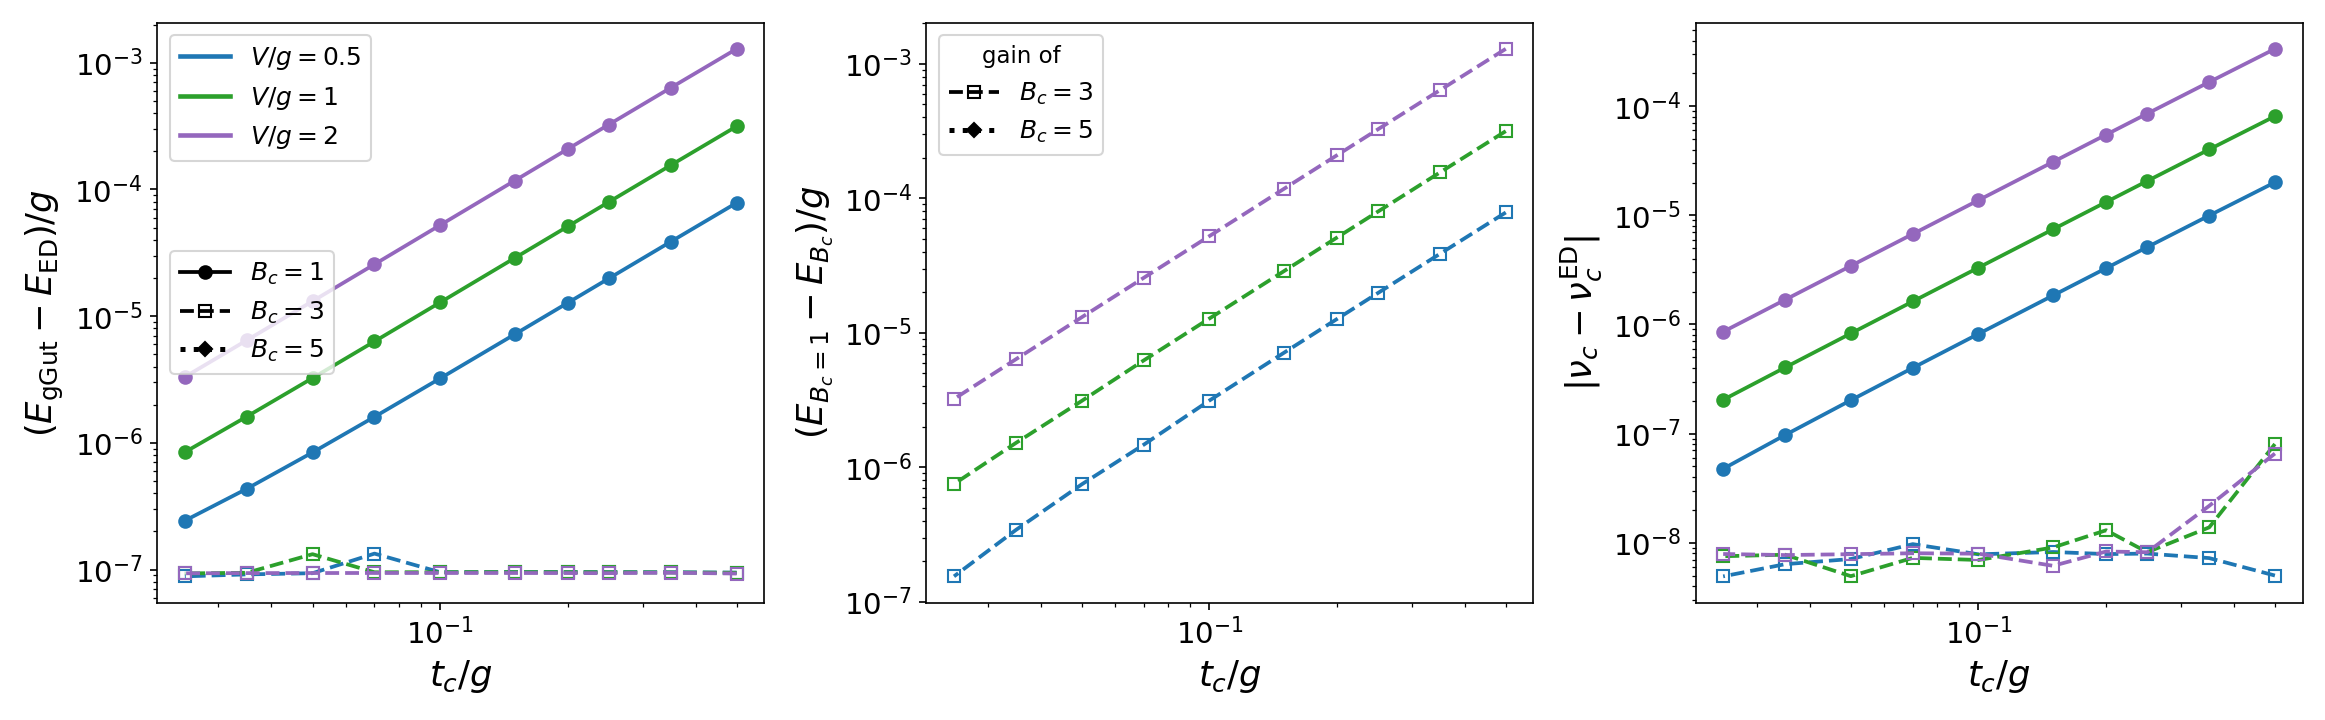
\includegraphics[width=\textwidth]{../cederbaum_data/cederbaum_energies.png}
  \caption{Left: $E_{\rm gGut}-E_{\rm ED}$ for $B_c=1$ (full lines), $B_c=3$ (dashed, open squares) and $B_c=5$ (dotted,
  diamonds); blue: $\rho/\Omega=0.5$ ($V/g=0.707$), purple: $\rho/\Omega=1.0$ ($V/g=1.414$). Middle: energy gained by the ghosts, $E_{B_c=1}-E_{B_c}$ (the two coincide).
  Right: $|\nu_c-\nu_c^{\rm ED}|$. Log--log axes; $E_c/g=10$.}
  \label{fig:energies}
\end{figure}

\begin{itemize}
\item \textbf{$B_c=1$:} $E_{\rm gGut}-E_{\rm ED}\simeq1.3\times10^{-3}\,V^2t_c^2$ over $t_c/g\in[0.025,0.5]$ (exponent $1.97$ and $1.99$), and $|\nu_c-\nu_c^{\rm ED}|\propto t_c^2$.
\item \textbf{$B_c=3$:} $E_{\rm gGut}-E_{\rm ED}=9.2$--$9.6\times10^{-8}$ for all $(V,t_c)$, flat; $|\nu_c-\nu_c^{\rm ED}|\le2.3\times10^{-8}$. This floor is the regularization shift, not the ansatz.
\item \textbf{$B_c=5$:} the same energy at all 20 points ($E_{B_c=5}-E_{B_c=3}$ between $-6\times10^{-11}$ and $+6\times10^{-13}$; KKT $\le2.3\times10^{-6}$); 5--9 of 14 runs per point converged to the same energy, and 3 of 120 random starts. The extra ghosts do not lower the energy.
\end{itemize}
The ghosts thus recover $79$--$99.99\%$ of the $B_c=1$ error (the smallest fractions at the smallest $t_c$, where the shift floor is comparable to the error).
Poor local minima from continuation ($(V/g,t_c/g)=(0.707,0.025)$, $(1.414,0.07)$) were recomputed from random starts; one $B_c=1$ loop point needed mixing $0.3$; two $B_c=5$ seeds were obtained by continuation.

\subsection{Hole spectral function}
\label{sec:spectra}

\begin{figure}[!ht]
  \centering
  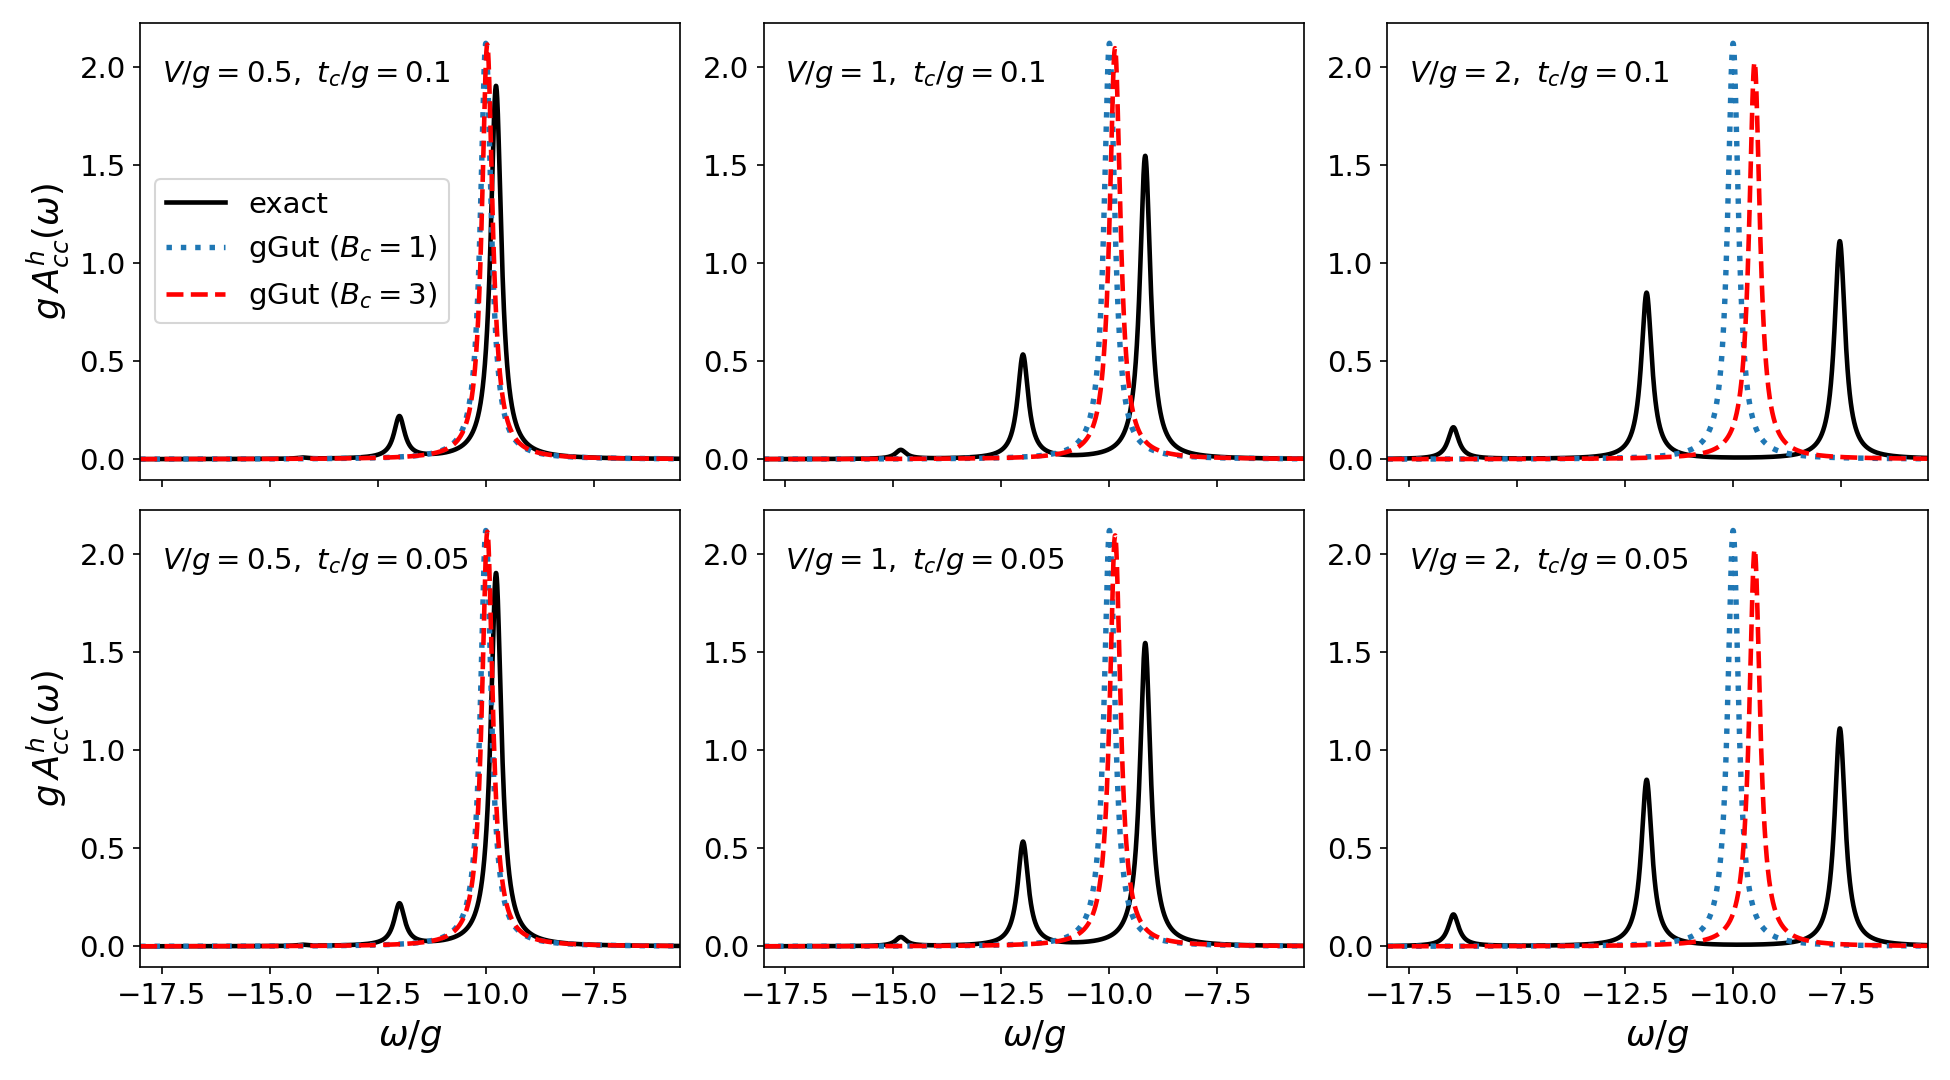
\includegraphics[width=\textwidth]{../cederbaum_data/cederbaum_spectra.png}
  \caption{Hole spectral function $A^h_{cc}(\omega)=\sum_n w_n\,(\eta/\pi)/[(\omega-\omega_n)^2+\eta^2]$, $\eta=0.15$: exact (solid), gGut $B_c=1$ (blue dotted), $B_c=3$ (red dashed), $B_c=5$ (green dotted, on top of $B_c=3$).
  Rows: $t_c/g=0.1$, $0.05$; columns: $\rho/\Omega=0.5$ ($V/g=0.707$), $1.0$ ($V/g=1.414$); $E_c/g=10$. Muted dots below zero: the zero-weight poles that the ghosts introduce (occupied ghost levels of $H_{qp}$), as returned by the minimizer:
  one at $B_c=3$ (small, rose), two at $B_c=5$ (large, green); $B_c=1$ has none. Their positions are not fixed by the solution (see text) and they carry no weight.}
  \label{fig:spectra}
\end{figure}

\begin{table}[!ht]
\centering\footnotesize
\setlength{\tabcolsep}{4pt}
\begin{tabular}{rr rr rr rr rr}
\toprule
 & & \multicolumn{2}{c}{ED main pole} & \multicolumn{2}{c}{gGut $B_c=1$} & \multicolumn{2}{c}{gGut $B_c=3$} & \multicolumn{2}{c}{gGut $B_c=5$}\\
$V/g$ & $t_c/g$ & position & weight & position & weight & position & weight & position & weight\\
\midrule
0.707 & 0.1  & $-9.5516$ & 0.8250 & $-10.0007$ & 0.9999 & $-9.9355$ & 0.9940 & $-9.9355$ & 0.9940\\
0.707 & 0.05 & $-9.5508$ & 0.8249 & $-9.9997$ & 0.9999 & $-9.9330$ & 0.9939 & $-9.9330$ & 0.9939\\
1.414 & 0.1  & $-8.5373$ & 0.6222 & $-10.0005$ & 0.9999 & $-9.7458$ & 0.9767 & $-9.7458$ & 0.9767\\
1.414 & 0.05 & $-8.5362$ & 0.6221 & $-9.9997$ & 0.9999 & $-9.7435$ & 0.9766 & $-9.7434$ & 0.9766\\
\bottomrule
\end{tabular}
\caption{Dominant hole pole of $G_{cc}$. ED additionally has satellites at about $-12.0$ (total weight $0.167$ and $0.333$ for $V/g=0.707$, $1.414$) and at $-14.45$ and $-15.47$ (weights $0.008$ and $0.045$);
gGut has none: all other occupied levels have weight $\le1.5\times10^{-6}$ ($B_c=1$) and $\le2.2\times10^{-6}$ ($B_c=3$, $5$).}
\label{tab:poles}
\end{table}

\paragraph{Result.} The $B_c=1$ pole sits at $-10.000$ for every $V$: the bare core level. At $B_c=3$ and $5$ (identical to $10^{-4}$) the single pole moves with $V$ towards the exact main pole but covers only $15$--$18\%$ of the exact displacement from $-E_c$
($0.067$ of $0.449$ and $0.257$ of $1.464$ at $t_c/g=0.05$), and its weight ($0.994$, $0.977$) stays far above the exact one ($0.825$, $0.622$). \emph{No satellites appear}; the ghosts only add $V$ dependence to the main pole.

\paragraph{Why there is no weight on the ghosts (interpretation).} The weights in Eq.~\eqref{eq:Ghgg} are $|R_c^T\phi^{(c)}_n|^2$. At $B_c=3$ ($t_c/g=0.1$) the natural orbitals of ${}^c\Delta$ have occupations $\sim10^{-7}$, $0.9999$ and $1$ (the nearly full core orbital and two pure ghosts),
and $R_c$ lies entirely along the core orbital (components along the others $\le10^{-4}$), so the occupied ghost level carries $3\times10^{-7}$ and $4\times10^{-10}$ at $V/g=0.707$, $1.414$ ($\le2.3\times10^{-9}$ at $B_c=5$), and $R_c^TR_c=0.994$, $0.977$ sits on one pole.
Mixing the two filled core orbitals by hand in $\lambda_c$ does split the weight (e.g.\ $0.57/0.42$ at $V/g=0.707$, $\delta=1$), but $\|[H_{qp},\rho]\|$ then grows from $\le2.6\times10^{-5}$ to $10^{-2}$--$4\times10^{-2}$: these points are not stationary, and their poles and weights do not match the exact ones.
The ghosts appear to carry the correlation through $\nu_c$ and $K$ (the terms $-V(\bar\Theta u)R_o^T$, $-V(\bar\Theta w)R_v^T$ of $H_{qp}$) but not through $R_c$, which is all that Eq.~\eqref{eq:Ghgg} sees.

\paragraph{The zero-weight ghost poles.} A level of $H_{qp}$ is a ghost pole if it is occupied in $\rho$ ($\ge0.5$), lies on the core-and-ghost block ($>0.99$) and has core weight $<10^{-4}$ (classified by occupation, not by energy order: a free ghost level can cross the valence level $o$).
There is one at $B_c=3$ and two at $B_c=5$; none at $B_c=1$. The other occupied level is the valence orbital $o$ (core weight $\le3\times10^{-6}$, at $\epsilon\simeq-g$), and $v$ is empty. As returned by the minimizer the ghost poles lie \emph{above} the QP peak,
at $+0.2$ to $+4.6\,\Omega$ (Figs.~\ref{fig:spectra}, \ref{fig:golze}). Their positions carry no information: the constraint Jacobian has rank $7$ of $8$ ($B_c=3$) and $13$ of $17$ ($B_c=5$), and shifting the multipliers along the undetermined directions moves them
(for example to the exact satellite energies) without changing $E$, the main pole, its weight or $\|[H_{qp},\rho]\|$, while their weights stay $\le8\times10^{-9}$, so no satellite appears; different minimizer solutions of the same point place them differently
(at $B_c=3$, $t_c/g=0.05$ the ghost level is at $-2.98$ and $-5.93$ in the solutions of the figures, $-2.20$ and $-9.53$ in earlier ones). The returned positions are the minimum-norm multipliers of the least-squares recovery.
Why they lie where they do: in gGut every pole of $G^h_{cc}$ is an eigenvalue of $H_{qp}$. The exact satellites are \emph{below} the main peak, at $-12$ and $-14.5$ ($V/g=0.707$) or $-15.5$ ($V/g=1.414$), against a main pole at $-9.6$ (exact) or $-9.9$ (gGut).
A ghost level could therefore only produce a satellite if it lay at $-12$ or lower, deeper than the core QP level and than every other level of $H_{qp}$. The energy of a ghost level, however, is not set by the core energy $E_c$: it comes from the multipliers of the density constraint, which are of valence-scale magnitude
(the bath levels of $\lambda^c_c$ at $t_c/g=0.5$ are $-2.1$ to $+1.7$ and $-5.1$ to $+3.0$; \texttt{excited\_phi\_cederbaum.tex}). The ghost levels therefore lie between the core level ($\approx-10$) and the valence region ($\approx-1$), i.e.\ \emph{above} the main peak, not below it.
Since the weight is set by $R_c$, which the energy minimization fixes along the core orbital, a solution with satellite weight would differ from the minimum; none was found.

\begin{figure}[H]
  \centering
  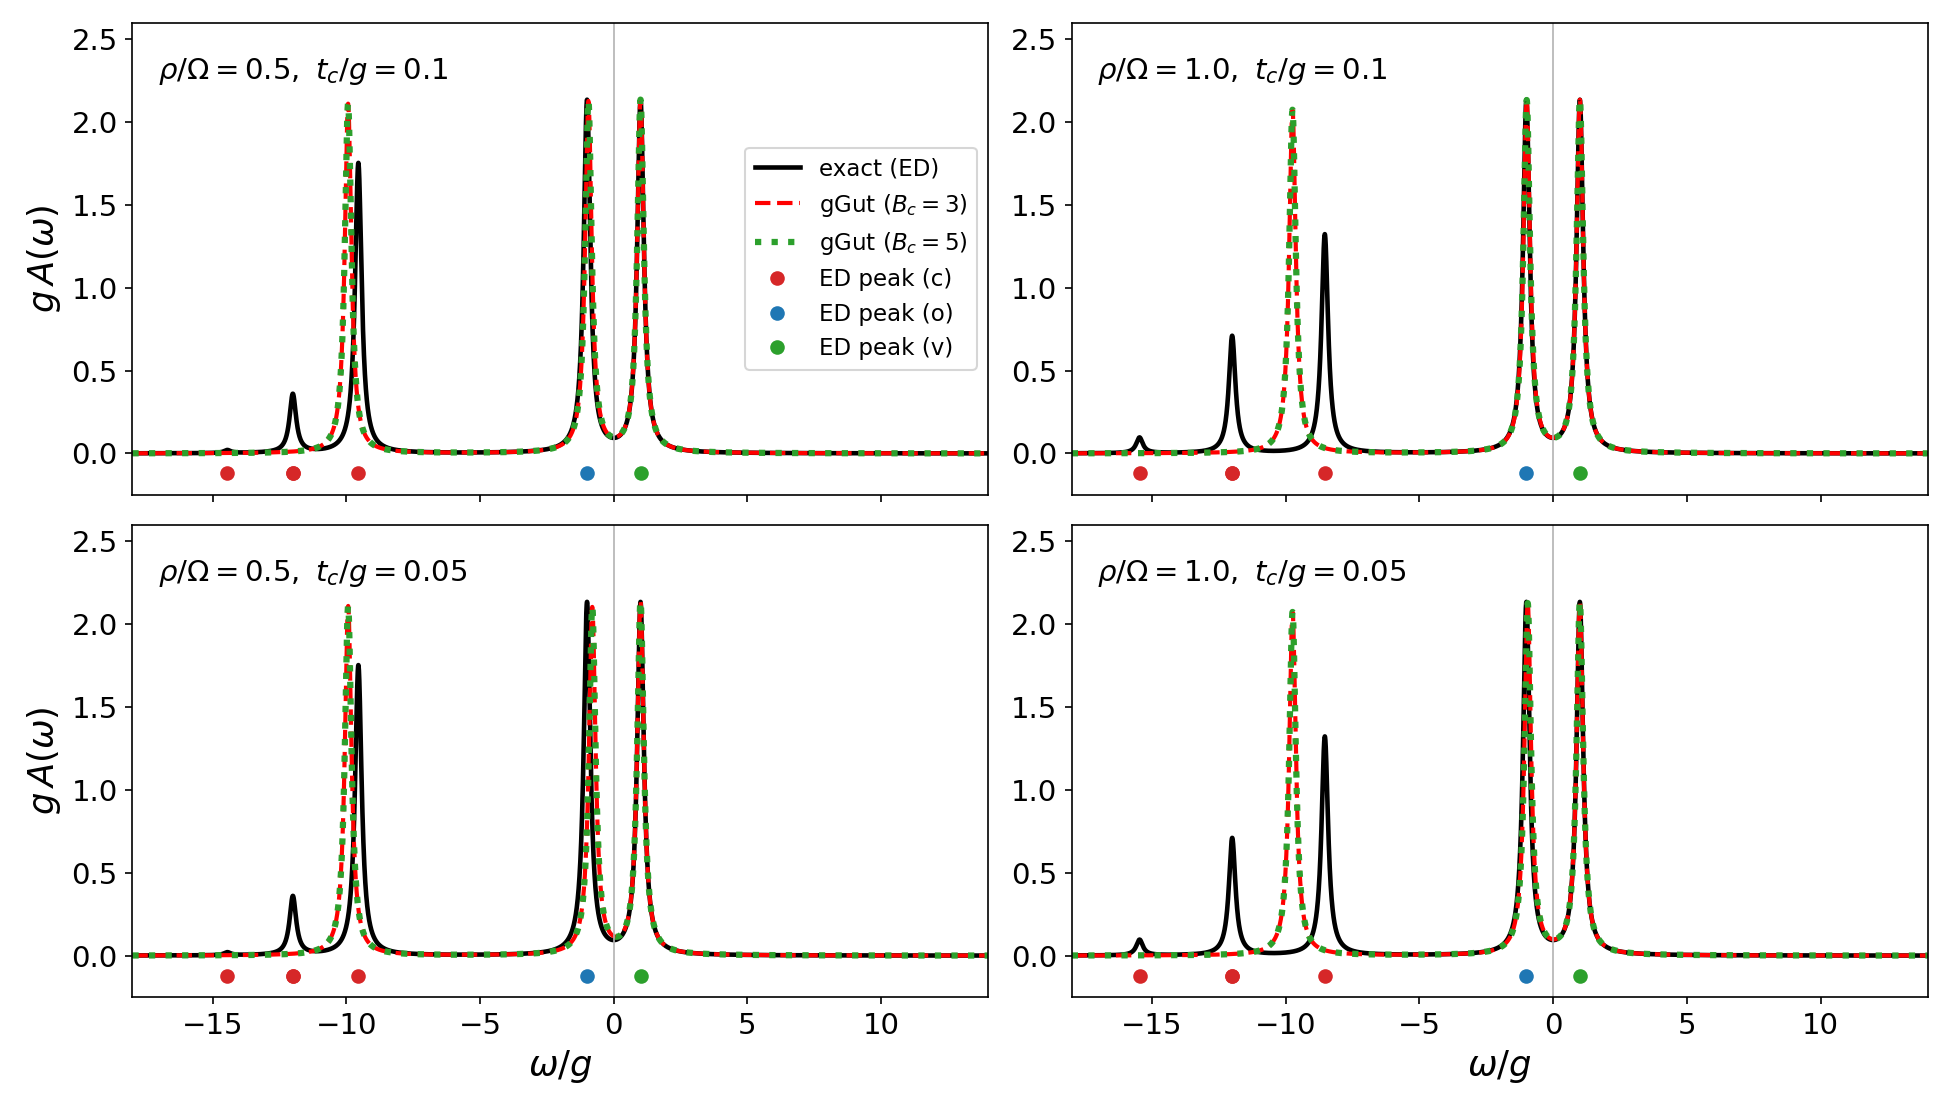
\includegraphics[width=\textwidth]{../cederbaum_data/cederbaum_fullspectra.png}
  \caption{Full spectral function $A(\omega)=\sum_{I=c,o,v}A_{II}(\omega)$ (hole and particle sides, per spin, $\eta=0.15$, $E_c/g=10$): exact (black), gGut $B_c=3$ (red dashed) and $B_c=5$ (green dotted), from the cached solutions of Fig.~\ref{fig:spectra}.
  Rows: $t_c/g=0.1$, $0.05$; columns: $\rho/\Omega=0.5$, $1.0$. Dots below the axis: ED peaks of weight $>10^{-3}$, coloured by orbital ($c$ red, $o$ blue, $v$ green).}
  \label{fig:fullspec}
\end{figure}

\paragraph{Full spectral function (core, occupied, virtual).}
Fig.~\ref{fig:fullspec} shows all peaks of $A=A_{cc}+A_{oo}+A_{vv}$, hole side ($\omega<0$) and particle side ($\omega>0$), against ED.
In gGut every eigenvalue of $H_{qp}$ is a pole, occupied ones on the hole side and empty ones on the particle side, with weight $|R_I^T\phi^{(I)}_n|^2$ on orbital $I$.
The three main peaks are the core hole near $-10$ ($c$), the occupied level near $-g$ ($o$) and the virtual level near $+g$ ($v$); gGut reproduces the last two, and the core pole only approximately (position and weight as in Tab.~\ref{tab:poles}).
What gGut misses are the exact core satellites at $-12$ and $-14.5$ ($-15.5$); the remaining ED peaks ($\omega\simeq3$ for $c$ and $\omega\simeq12$ for $o$, particle side) have weight $\lesssim10^{-6}$ and are not visible.
The extra gGut levels ($B_c=3$: one at $-5.9$ to $-3.0$, $B_c=5$: several between $-4.7$ and $+1.4$, plus the empty level at $\simeq+12$) are ghost levels with weight $\le10^{-4}$.

\subsection{Comparison with the three-level model of Cederbaum and of Kockl\"auner and Golze}
\label{sec:golze}

The orbitals $c$, $o$, $v$ are the three-level core-hole model of Cederbaum, Domcke and Schirmer~\cite{Cederbaum1980} (Eqs.~(28)--(29)), used by Kockl\"auner and Golze~\cite{Kocklauner2024} (Fig.~2) to test G$_0$W$_0$ and GW plus cumulant (GW+C).
With $\Omega=\epsilon_v-\epsilon_o=2g$ and the transition moment $\rho$ (GW+C excitation weight $\gamma=\rho^2/\Omega^2$), the exact solution is the $3\times3$ matrix with off-diagonal elements $-\sqrt2V$, which gives Eq.~\eqref{eq:poles} and the weights $(a\pm\Omega)^2/4a^2$, $2V^2/a^2$ of Ref.~\cite{Cederbaum1980}
($a=(\Omega^2+4V^2)^{1/2}$). The $\sqrt2$ is the normalization of the two spin channels, so
\begin{equation}
\rho=\sqrt2\,V,\qquad \frac{\rho}{\Omega}=\frac{V}{\sqrt2\,g},
\end{equation}
confirmed by the small-$V$ limit of the exact satellite-to-QP weight ratio ($2.00\times10^{-4}=(\sqrt2V)^2/\Omega^2$ at $V/g=0.02$, \texttt{g0w0\_cederbaum.py}). Their ratios $\rho/\Omega=0.5$, $1.0$ are $V/g=0.707$, $1.414$, the values used throughout this note.
Their figure gives only the ratio, no energy axis, so $E_c$ cannot be taken from it (it only shifts the poles rigidly); Fig.~\ref{fig:golze} plots $(\omega-\epsilon_{\rm QP})/\Omega$.

\paragraph{G$_0$W$_0$ and GW+C for the model (computed here).} We computed G$_0$W$_0$ and GW+C for this model ourselves (\texttt{g0w0\_cederbaum.py}) from the expressions below, in order to compare with the G$_0$W$_0$ and GW+C of Ref.~\cite{Kocklauner2024} (not taken from it). With $G_0$ the bare core level and one bosonic mode, $\Sigma_c(\omega)=\rho^2/(\omega-\epsilon_c+\Omega)$ (no exchange or Hedin shift), the poles of $[\omega-\epsilon_c-\Sigma_c]^{-1}$ solve $x(x+\Omega)=\rho^2$: a QP pole and one satellite at $-\Omega\sqrt{1+4\rho^2/\Omega^2}$,
against the exact satellites at $-\Omega\sqrt{1+2\rho^2/\Omega^2}$ and twice that. GW+C has Poisson satellites at $\epsilon_{\rm QP}-n\Omega$ with weights $e^{-\gamma}\gamma^n/n!$. These expressions agree with Eqs.~(11), (14), (16)--(17), (33), (36), (44)--(47) of Ref.~\cite{Kocklauner2024} (the exchange constant $\Sigma^x-v^{xc}$ is absorbed in $\epsilon_c$),
and the first-satellite positions measured in their rendered Fig.~2b,c (in units of $\Omega$, accuracy a few per cent) agree with this note: exact $1.22$ and $1.76$ (here $1.225$, $1.732$), G$_0$W$_0$ $1.42$ and $2.23$ (here $1.414$, $2.236$) at $\rho/\Omega=0.5$, $1.0$.

\begin{table}[!ht]
\centering\footnotesize
\begin{tabular}{r l l l}
\toprule
$\rho/\Omega$ & & satellite positions $/\Omega$ (from QP) & weights (QP, satellites)\\
\midrule
0.5 & exact & $-1.225$, $-2.449$ & $0.825$, $0.167$, $0.008$\\
    & G$_0$W$_0$ & $-1.414$ & $0.854$, $0.146$\\
    & GW+C & $-1$, $-2$, $-3,\dots$ & $0.779$, $0.195$, $0.024,\dots$\\
1.0 & exact & $-1.732$, $-3.464$ & $0.622$, $0.333$, $0.045$\\
    & G$_0$W$_0$ & $-2.236$ & $0.724$, $0.276$\\
    & GW+C & $-1$, $-2$, $-3,\dots$ & $0.368$, $0.368$, $0.184,\dots$\\
\bottomrule
\end{tabular}
\caption{Exact ($t_c=0$), G$_0$W$_0$ and GW+C hole spectrum of the model at the ratios of Fig.~2 of Ref.~\cite{Kocklauner2024} ($V/g=0.707$, $1.414$).}
\label{tab:golze}
\end{table}

\begin{figure}[!ht]
  \centering
  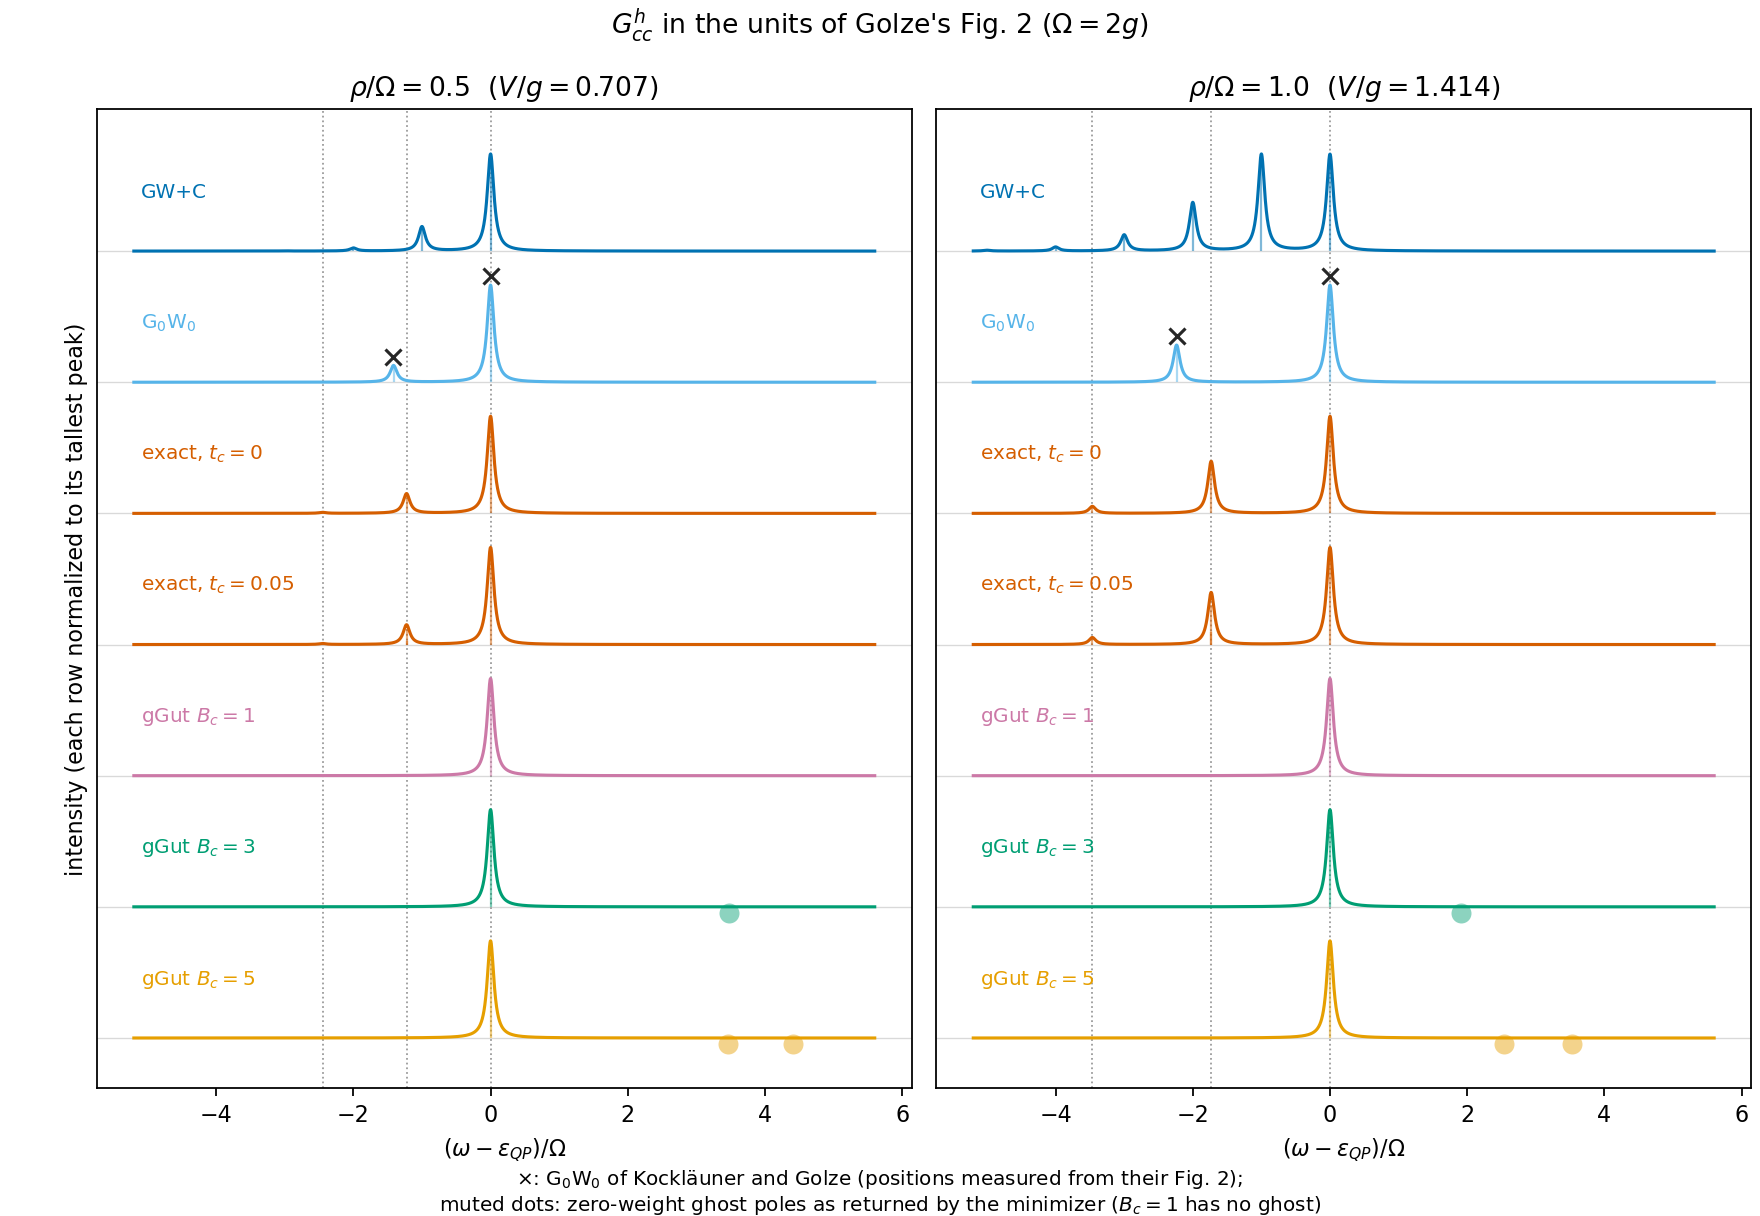
\includegraphics[width=\textwidth]{../cederbaum_data/golze_units.png}
  \caption{$G^h_{cc}$ in the units of Fig.~2 of Ref.~\cite{Kocklauner2024} (Lorentzian width $0.06\,\Omega$; each row normalized to its tallest peak); left $\rho/\Omega=0.5$ ($V/g=0.707$), right $\rho/\Omega=1.0$ ($V/g=1.414$), $E_c/g=10$.
  Rows: GW+C; G$_0$W$_0$ (computed here from the model, Eqs.\ below, to match the G$_0$W$_0$ of Ref.~\cite{Kocklauner2024}); exact at $t_c=0$ and $0.05$; gGut $B_c=1$, $3$, $5$ ($t_c/g=0.05$). Dotted lines: the exact poles at $t_c=0$. Crosses ($\times$): the G$_0$W$_0$ of Kockl\"auner and Golze (QP peak and satellite), positions measured from their rendered Fig.~2 ($-1.42\,\Omega$ and $-2.23\,\Omega$; accuracy $\sim2\%$, \texttt{measure\_golze\_fig2.py}); our computed G$_0$W$_0$ reproduces them. gGut has a single peak at every $B_c$. Muted dots: the zero-weight ghost poles as returned by the minimizer (one at $B_c=3$, two at $B_c=5$, none at $B_c=1$),
  at positive $(\omega-\epsilon_{\rm QP})/\Omega$ and without weight.}
  \label{fig:golze}
\end{figure}

\paragraph{What matches.} The exact spectrum has the QP peak and two satellites (a single and a double $o\to v$ excitation, the second much weaker), with intensity and QP--satellite separation growing with $\rho/\Omega$; G$_0$W$_0$ has one satellite at higher binding energy than the exact one
($-1.41\,\Omega$ against $-1.23\,\Omega$ at $\rho/\Omega=0.5$; $-2.24\,\Omega$ against $-1.73\,\Omega$ at $1.0$); GW+C puts satellites at $-n\Omega$ (closer to the exact ones at $\rho/\Omega=0.5$ than at $1.0$) and shows spurious higher satellites at larger $\rho/\Omega$; all as stated in Ref.~\cite{Kocklauner2024}. The hopping $t_c$ moves the exact poles by at most $0.06$ at $t_c/g=0.5$.

\paragraph{What does not match.} gGut gives a single pole at both ratios (weight $0.977$--$0.9999$): it reproduces neither the exact satellites nor the GW+C or G$_0$W$_0$ ones, and does worse than G$_0$W$_0$ for this model, whose QP pole is within $0.04$ and $0.23$ of the exact one ($-9.59$, $-8.76$ against $-9.55$, $-8.54$)
while the gGut $B_c=3$ pole is at $-9.93$, $-9.74$ (errors $0.38$, $1.21$) and the $B_c=1$ pole at $-10.00$. The ghost poles (muted dots) are not satellites: no weight and arbitrary positions, as discussed above.

%======================================================================
\section{Conclusions}
\label{sec:conclusion}

\begin{enumerate}
\item \textbf{gGut does not reproduce the satellite structure of the model.} For $B_c=1$, $3$, $5$, $\rho/\Omega=0.5$, $1.0$ ($V/g=0.707$, $1.414$) and $t_c/g=0.05$--$0.5$, the hole spectral function has a single pole with weight $0.977$--$0.9999$, whereas the exact spectrum has satellites near $-12$ and at $-14.45$, $-15.47$ carrying $17.5\%$ and $37.8\%$ of the weight.
The main pole is displaced from the exact one ($-9.93$ vs.\ $-9.55$; $-9.74$ vs.\ $-8.54$).
\item The ghosts improve the ground state: $E-E_{\rm ED}\approx10^{-7}$ at $B_c=3$ and $5$ (vs.\ $1.3\times10^{-3}V^2t_c^2$ at $B_c=1$), $\nu_c$ to $\sim10^{-8}$; $B_c=5$ returns the $B_c=3$ energy and spectrum (the extra ghosts stay asleep).
\item The extra occupied ghost levels have zero weight ($R_c$ lies along the core orbital) and arbitrary energy (free multiplier directions): moving them to the exact satellite energies leaves $E$ and the weights unchanged, so they give no satellite. A solution with satellite weight would have to change $R_c$, i.e.\ differ from the energy minimum; none was found.
\item The model uses a core--virtual hopping: a core--occupied hopping leaves $\ket{220}$ exact for every $t_c$ and cannot make $R_c$ determined. The energy functional and its gradients are verified (finite differences $\sim10^{-10}$), and the limits $V=0$, $t_c=0$ are reproduced.
\item The model is the three-level model of Cederbaum \emph{et al.}~\cite{Cederbaum1980} with $\rho=\sqrt2V$; for $\rho/\Omega=0.5$, $1.0$ the exact spectrum has the QP peak and two satellites, G$_0$W$_0$ one satellite at too high a binding energy, GW+C satellites at $-n\Omega$, and gGut a single pole (Fig.~\ref{fig:golze}, Tab.~\ref{tab:golze}).
\end{enumerate}

%======================================================================
\appendix
\section{The quasiparticle Hamiltonian as a matrix}
\label{sec:appHqp}

$H_{qp}$ acts on the $B_c+2$ quasiparticle orbitals of one spin, ordered as the $B_c$ core orbitals $d_{c1},\dots,d_{cB_c}$, then $d_o$, then $d_v$
(the block structure ${\rm c},{\rm o},{\rm v}$ of $\rho$ in Sec.~\ref{sec:gGut}). It is real and symmetric. Its ingredients, all defined in Sec.~\ref{sec:gGut}, are the
renormalization vectors $R_c\in\mathbb R^{B_c}$, $R_o,R_v\in\mathbb R$, the core occupation $\nu_c$, the tensor $\bar\Theta\in\mathbb R^{B_c\times B_c}$
and the two core vectors
\begin{equation}
a=\bar\Theta\,u=\bar\Theta\,\rho^{cv}R_v,\qquad b=\bar\Theta\,w=\bar\Theta\,\rho^{co}R_o\qquad(a,b\in\mathbb R^{B_c}).
\end{equation}
The diagonal blocks are the multipliers of the constraint $\rho^{II}={}^I\Delta$ of Eq.~\eqref{eq:problem}, $-\lambda_c\in\mathbb R^{B_c\times B_c}$ (symmetric) and
$-\lambda_o,-\lambda_v\in\mathbb R$; the off-diagonal blocks are $H^{IJ}=\tfrac14\partial E/\partial\rho^{IJ}$ of Sec.~\ref{sec:direct}. In block form, with the blocks of
size $B_c$, $1$, $1$,
\begin{equation}
H_{qp}=
\begin{pmatrix}
-\lambda_c & -V R_o\,a & R_v\,(t_cR_c-V\,b)\\[2pt]
-V R_o\,a^T & -\lambda_o & -V(2-\nu_c)\,R_oR_v\\[2pt]
R_v\,(t_cR_c-V\,b)^T & -V(2-\nu_c)\,R_oR_v & -\lambda_v
\end{pmatrix}.
\label{eq:Hqpblock}
\end{equation}
The $co$ and $cv$ blocks are the column vectors $-VR_o\,a$ and $R_v(t_cR_c-Vb)$ ($B_c\times1$); the $ov$ block is a number.
This is what \texttt{build\_Hqp} returns (\texttt{gga\_cederbaum.py}), and it is the same operator as $H_{\rm off}-\mathrm{blockdiag}(\lambda_I)$ of Sec.~\ref{sec:direct}.

\paragraph{Spin.} $H_{qp}$ and $\rho$ in this appendix are the \emph{one-spin} matrices, of size $B_c+2$: $\rho_{pq}=\braket{d\dg_{p\sigma}d_{q\sigma}}$ with $\sigma$ fixed, and the
solutions are paramagnetic, so $\uparrow$ and $\downarrow$ have the same matrix. The quasiparticle Hamiltonian on the full space of $2(B_c+2)$ spin orbitals, ordered
$(\uparrow\text{ block},\downarrow\text{ block})$, is
\begin{equation}
H_{qp}^{\rm full}=\begin{pmatrix}H_{qp}&0\\0&H_{qp}\end{pmatrix}=\mathbb 1_2\otimes H_{qp},\qquad
\rho^{\rm full}=\mathbb 1_2\otimes\rho ,
\end{equation}
and each spin channel fills its $N_{\rm occ}$ lowest levels ($N_{\rm occ}=2$ for $B_c=1$, $3$ for $B_c=3$), i.e.\ $2N_{\rm occ}$ electrons in total. The spin sum and the hermitian conjugate that give the factor $4$ in Eq.~\eqref{eq:E}
are removed in $H^{IJ}=\tfrac14\partial E/\partial\rho^{IJ}$, so the entries below carry no spin factor.

\paragraph{Explicit form for $B_c=1$.} There are no ghosts, $\lambda_c$, $a$, $b$, $R_c$, $\bar\Theta$ are numbers and $H_{qp}$ is $3\times3$:
\begin{equation}
H_{qp}^{B_c=1}=
\begin{pmatrix}
-\lambda_c & -V R_o\,a & R_v(t_cR_c-V\,b)\\
-V R_o\,a & -\lambda_o & -V(2-\nu_c)R_oR_v\\
R_v(t_cR_c-V\,b) & -V(2-\nu_c)R_oR_v & -\lambda_v
\end{pmatrix},
\end{equation}
with $a=\bar\Theta R_v\rho^{cv}$ and $b=\bar\Theta R_o\rho^{co}$.

Diagonalizing it, $H_{qp}\phi_n=\epsilon_n\phi_n$ ($\epsilon_1\le\epsilon_2\le\epsilon_3$, $\phi_{n,p}$ the component of $\phi_n$ on orbital $p$), and filling the
$N_{\rm occ}=2$ lowest levels per spin gives $\rho_{pq}=\braket{d\dg_{p\sigma}d_{q\sigma}}=\sum_{n=1}^{2}\phi_{n,p}\phi_{n,q}\equiv s_{pq}$:
\begin{equation}
\rho^{B_c=1}=
\begin{pmatrix}
s_{cc}&s_{co}&s_{cv}\\ s_{co}&s_{oo}&s_{ov}\\ s_{cv}&s_{ov}&s_{vv}
\end{pmatrix}.
\end{equation}
The diagonal entries are the new ${}^I\Delta$, and the off-diagonal ones give the $a$, $b$ of the next $H_{qp}$ through $u=R_vs_{cv}$, $w=R_os_{co}$:
$a=\bar\Theta R_vs_{cv}$, $b=\bar\Theta R_os_{co}$.

\paragraph{Explicit form for $B_c=3$.} With $\lambda_c=(\lambda_{ij})$ symmetric, $a=(a_1,a_2,a_3)^T$, $b=(b_1,b_2,b_3)^T$, $R_c=(R_{c1},R_{c2},R_{c3})^T$ and
$\tau_i=t_cR_{ci}-Vb_i$, $H_{qp}$ is $5\times5$:
\begin{equation}
H_{qp}^{B_c=3}=
\begin{pmatrix}
-\lambda_{11} & -\lambda_{12} & -\lambda_{13} & -VR_oa_1 & R_v\tau_1\\
-\lambda_{12} & -\lambda_{22} & -\lambda_{23} & -VR_oa_2 & R_v\tau_2\\
-\lambda_{13} & -\lambda_{23} & -\lambda_{33} & -VR_oa_3 & R_v\tau_3\\
-VR_oa_1 & -VR_oa_2 & -VR_oa_3 & -\lambda_o & -V(2-\nu_c)R_oR_v\\
R_v\tau_1 & R_v\tau_2 & R_v\tau_3 & -V(2-\nu_c)R_oR_v & -\lambda_v
\end{pmatrix}.
\end{equation}

Diagonalizing it ($\epsilon_1\le\dots\le\epsilon_5$) and filling the $N_{\rm occ}=3$ lowest levels per spin gives
$\rho_{pq}=\sum_{n=1}^{3}\phi_{n,p}\phi_{n,q}\equiv s_{pq}$:
\begin{equation}
\rho^{B_c=3}=
\begin{pmatrix}
s_{c_1c_1}&s_{c_1c_2}&s_{c_1c_3}&s_{c_1o}&s_{c_1v}\\
s_{c_1c_2}&s_{c_2c_2}&s_{c_2c_3}&s_{c_2o}&s_{c_2v}\\
s_{c_1c_3}&s_{c_2c_3}&s_{c_3c_3}&s_{c_3o}&s_{c_3v}\\
s_{c_1o}&s_{c_2o}&s_{c_3o}&s_{oo}&s_{ov}\\
s_{c_1v}&s_{c_2v}&s_{c_3v}&s_{ov}&s_{vv}
\end{pmatrix}.
\end{equation}
The upper-left $3\times3$ block is the new ${}^c\Delta$ and $s_{oo}$, $s_{vv}$ the new ${}^o\Delta$, ${}^v\Delta$. The off-diagonal entries give the $a$, $b$ of the next
$H_{qp}$: $u=R_v(s_{c_1v},s_{c_2v},s_{c_3v})^T$, $w=R_o(s_{c_1o},s_{c_2o},s_{c_3o})^T$, $a=\bar\Theta u$, $b=\bar\Theta w$.

For $B_c=5$ the core block is $5\times5$ and the two border columns have five entries each, same pattern.

\paragraph{Use in the impurity loop.} In the impurity loop (\texttt{gga\_cederbaum.py}) $H_{qp}$ is diagonalized once per macroiteration; there is no inner loop on $\rho$.
The $\rho$ obtained from the occupied eigenvectors is used directly in the next macroiteration: its diagonal blocks $\rho^{II}$ are the ${}^I\Delta$ that
enter the embedding problems (before the linear mixing with their output), and its off-diagonal blocks give $u$, $w$ and hence $a$, $b$ in the next $H_{qp}$.
$\rho$ is thus self-consistent with $H_{qp}$ only at convergence of the macroiterations. (Repeating the diagonalization until $\rho$ stops changing, before the embedding step, was tested
and does not change the converged result for $B_c=1$ nor make the $B_c=3$ loop converge.)

In the direct minimization (Sec.~\ref{sec:direct}) no such cycle is needed: $\rho=X(X^TX)^{-1}X^T$ is a variable of the minimization, $E$ already contains the dependence of $H_{qp}$ on $\rho$
through $u$ and $w$, and the condition that $\rho$ is built from its own $H_{qp}$ is the stationarity condition $[H_{qp},\rho]=0$; the link $\rho^{II}={}^I\Delta(\Phi_I)$ is an equality constraint.
At the minimizers found, building $H_{qp}$ from the multipliers and from this $\rho$, diagonalizing it and filling the $N_{\rm occ}$ lowest levels returns the same $\rho$ to the accuracy of the stationarity
($\|\rho_{\rm filled}-\rho\|=10^{-8}$ for $B_c=1$ and for $B_c=3$ at $\varepsilon=10^{-5}$; $2\times10^{-5}$ for $B_c=3$ at $\varepsilon=10^{-9}$, where $\|[H_{qp},\rho]\|=3\times10^{-4}$), and the occupied levels are the lowest ones,
with a gap $1$--$2$ to the first empty level ($V/g=1$, $t_c/g=0.5$).

\begin{thebibliography}{9}
\bibitem{Cederbaum1980} L.~S. Cederbaum, W. Domcke and J. Schirmer, Many-body theory of core holes, Phys.\ Rev.\ A \textbf{22}, 206 (1980).
\bibitem{Kocklauner2024} J. Kockl\"auner and D. Golze, GW plus cumulant approach for predicting core-level shake-up satellites in large molecules, arXiv:2412.17132 (2024).
\end{thebibliography}

\end{document}
